\documentclass[12pt]{report} %12pt font and article style

\usepackage{graphicx} %to import pictures if necessary
\graphicspath{ {images/} }
\usepackage{amsmath} %to allow math symbols to show up
\usepackage{fullpage}
\setlength\parindent{24pt}

\begin{document}
\begin{titlepage}
%I 'borrowed' this title page example from: https://en.wikibooks.org/wiki/LaTeX/Title_Creation
\centering
    {\scshape\LARGE University of Prince Edward Island\par}
    \vspace{1cm}
    {\scshape\Large Honours Thesis\par}
    \vspace{1.5cm}
    {\huge\bfseries Fashion Forward-Propagation: Machine Learning Tackles Fashion Curation\par}
    \vspace{2cm}
    {\Large\itshape Hailey LeClair\par}
    \vfill
    supervised by\par
    Dr.~Andrew \textsc{Godbout}

\vfill

\today\par

\end{titlepage}
\tableofcontents
\newpage
\listoffigures
\newpage


\chapter{Introduction}
	Imagine an up and coming clothing designer with a small boutique. They have a small inventory of about 100 different items, and only carry a few different types of items. The items are dresses, shirts, shoes, and jeans. The designer wants to provide their customers with an easy way to find the clothing they make. To do this, they want to use an app in which the user can take a photo of any clothing item, and if the boutique has an item that looks similar, that item will be shown to the customer. Is this feasible for a small boutique with minimal technical resources? Can a computer that has five images of different dresses take another image of one of these dresses and find its match? This paper will attempt at answering these questions by exploring how an app like this might be possible using convolutional neural networks, and how a designer with minimal technical knowledge could use this sort of app.
	
	To look at this problem on a very high level, let us assume we have already created an app for these purposes. The designer would need to provide the app with several images of each of their items, so that this app, can learn things about these items within the image. As humans, we can easily distinguish the defining features of an object by looking at the object itself, or by looking at an image of the object. Without turning this into a biology paper, the neurons in our brain that are connected to our eyes are very intelligent and complex, and can recognize certain features of objects and objects themselves\cite{aurelienMachineLearning}. For example, in two different images, we can easily recognize a similar red dress on two different women with different body shapes, in different positions, with different scenery around them in the images. For a computer, it is not so easy. 
	
\begin{figure}
\centering
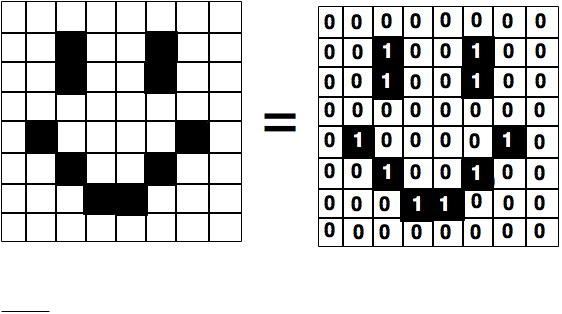
\includegraphics[width=4in]{pixels} 
\caption{A simple black and white image represented by pixel values 0 and 1}
\label{Fig: SimpleBWPixels}
\end{figure}
	
\section{Images}
%CHECK THIS THING ABOUT GREYSCALE VALUE
	To understand how it might be possible for a computer to recognize a dress in an image we must first understand how an image is represented on a computer. Computers see images as two dimensional data structures of pixels, as in the image on the left of Figure 1. Each pixel has a numeric value. In this simple image, each pixel is either 0 or 1, representing either white or black pixels, respectively. A greyscale image can similarly be represented, where the value is a number between 0 and 255, but larger, and images in colour are obviously a lot more complicated than this trivial example. They often have hundreds or thousands of pixels and each pixel is represented by an RGB (red, green, and blue) value. RGB values are a set of 3 values each of which is a number from 0 to 255. Because an RGB pixel has 3 values, and an image is already a two dimensional structure, RGB images are seen as 3 dimensional by a computer. For this reason, images take more processing power than many other types of data. \cite{szeliski2010computer}. 
	
	The field of computer vision emerged in the early 1970's as an attempt to get a computer to process and view digital images in the same way our brain and eyes do. In 1966, a professor at MIT asked a student to spend the summer with a camera connected to a computer, and to get the computer to explain what it was seeing through the camera. This kind of experiment was bound to fail with the state of technology in 1966, but led to much more research into how images can be represented digitally, how scenes are perceived visually, and how objects are recognized in a scene or image. Much of this research was done using 3D mathematical modelling, algorithms for digital image processing, and image and scene analysis. \cite{szeliski2010computer}

\section{Objects in Images}

	Since the idea here is to take an image, classify it, and find its match amongst a set of similar photos, this means that we need to be able to recognize the object in another context in another image, which is exactly what is done in the field of computer vision. Rigid, articulated, and deformable objects all need to be considered when doing object detection, recognition, or classification in images. In terms of physics, a rigid object is a body in which "the distance between any two given points on [the] rigid body remains constant in time regardless of external forces exerted on it "\cite{RigidBodyWiki}. In terms of images, this means that a rigid object will always have the same dimensions, or some translation of the same dimensions, in any given photo taken of this object. There exist many methods discovered within the field of computer vision to recognize rigid objects in an image, one of which is Scale Invariant Feature Transform (SIFT)\cite{lowe1999object}. 
	
	SIFT can recognize any objects which do not vary, based on image rotation, scaling, or translation (rigid objects). It also does well with different kinds of lighting and illumination, as well as 3D projection\cite{lowe1999object}. The "key" to SIFT, is something called "key localization". Key localization chooses "key locations at maxima and minima of a difference of Gaussian function applied in scale space."\cite{lowe1999object}. The term "scale space" is used here, because any scaling of the image will not effect the locations selected during this process. Without delving too deeply into SIFT, this process is possible by building image pyramids at different levels of scaling. These pyramids make the locations very stable, which aids greatly in recognizing objects in an image.\cite{lowe1999object}.

	This is a step in the right direction in the attempt to recognizing clothing in images. Theoretically, if we already have something in place that can take an image and tell us what category of clothing an object belongs to, we can then use these methods like SIFT to match rigid objects like shoes. It is tremendously useful that we have access to methods, but is the same type of object detection possible for clothing that changes shape because of the articulated nature of the human body? Can we recognize a deformable dress that looks completely different on the hanger than it does while being worn? To attempt to answer these questions, we need to look at the possibilities surrounding these difficult types of objects. 
	
	Articulated objects may have rigid parts, but like human body parts, are connected at a basic joint which can move\cite{szeliski2010computer}. Multiple images of the same articulated object may show the object in different formations or positions. Although parts of these objects are rigid, possible movements from the joints mean that many different positions are possible for one articulated object. Think of all the possibilities of position for a human arm. An arm can be up in the air, straight out to the side, hanging down by the side of the body, bent at the elbow, behind the back, just to list a few. Even though articulated objects are rigid to a point, or, a joint, the degrees of freedom involved with these objects mean they are much more difficult to detect in images.
	
 \begin{figure}
\centering
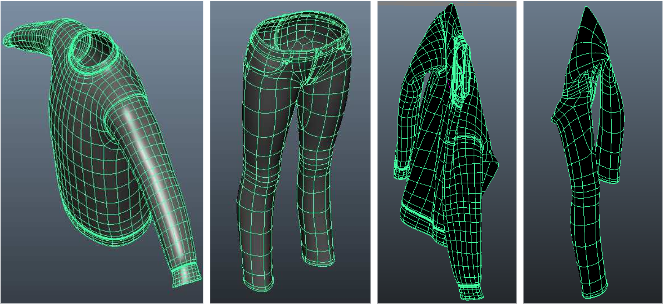
\includegraphics[width=4in]{deformable} 
\caption{Clothing shown as a Deformable Object}
\end{figure}

	A deformable object, in contrast with the others, "changes its shape and/or volume while being acted upon by any kind of external force"\cite{wolfram}. Depending on the degree to which an object deforms, or the amount of force applied, many images of an object could show it as having completely different dimensions and shape. As with articulated objects, the uncertainty of the general shape or dimensions makes deformable objects especially challenging. This problem, and the problem with articulated objects is particularly relevant with clothing. 
	
	With some exceptions (like shoes, jewelry, some accessories, for example), many everyday clothing items are deformable to some degree. For instance, a pair of skinny jeans may have a general shape when lifeless on a hanger, but take on very different dimensions and possibly even a totally different shape when being worn by different people. Like these jeans, of course, many other clothing items will take on the shape of the person wearing them. An example of this is shown in figure 2.\cite{Li_ICRA2014} In terms of shape and dimension of these two clothing items being worn and not being worn, there are barely any similarities. We can also consider changes in an environment that could change the shape of an object. If it is a particularly windy day, a long flowing dress may take on a completely different shape in the wind.

	As mentioned earlier, clothing items are typically being worn by someone in images. This simple fact adds one extra dimension to the recognition of any given clothing item, because the human body is an articulated body. A loose denim jacket, which may have a similar shape on anyone who wears it, can be easily deformed by placing the arms in a different position. Different articulations of the joints in the human body (especially our knees, shoulders, and elbows) can dramatically affect the shape and dimensions of a piece of clothing, and this carries over to the digital image. These obstacles add a layer to object recognition in clothing items, which would not be present in recognizing various other types of objects in images. Unfortunately, we cannot rely on something like SIFT\cite{lowe1999object} to recognize these sorts of items in an image, as it struggles to detect these nuances. 


	Along with the problem of clothing being deformable and worn on an articulated body, we also have to consider the other contextual aspects of an image. As intelligent humans, we can normally determine if a dress in an image is the same as another dress in another image, regardless of what other objects are in the background. When it comes to digital recognition, though, an image containing an explicit clothing item could be convoluted with other objects or people in the same image, or could have an explicit, plain background which becomes a defining feature of an image. When introduced to another image of the same object with a similarly noisy background, a computer may then think this is a different object altogether, because of the dramatic difference in backgrounds between this photo and the previous one(s). 
	%https://www.sneakersfansno.com/product_info.php?c=nike%20roshe%20one%20men
	%https://www.jumia.com.ng/nike-roshe-one-men-black-shoes-6815562.html
	
	
\section{Other Difficulties in Object Recognition in images}
\begin{figure}
\centering
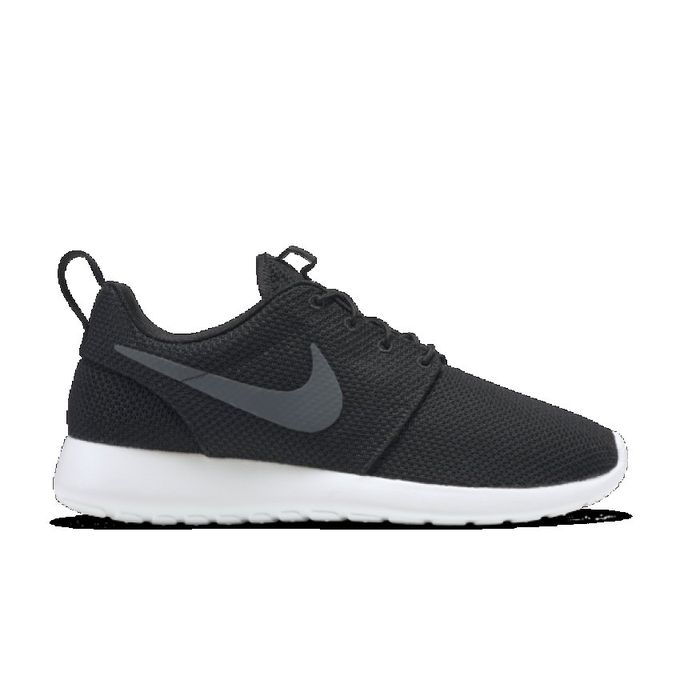
\includegraphics[width=4in]{nike} 
\centering
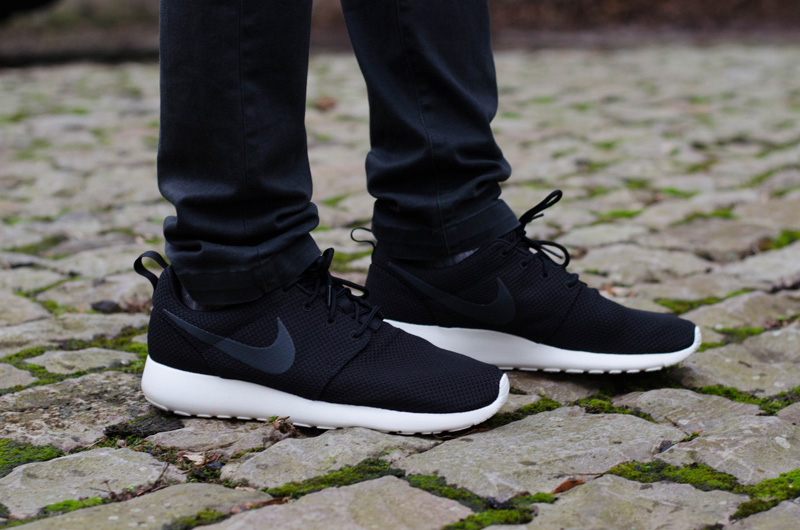
\includegraphics[width=4in]{nike_on_man} 
\caption{Two photos of Nike Rosch One sneaker. One being worn by a person on cobblestone, and one with a white background}
\end{figure}
	
	Figure 3 shows the same nike shoe in two different images. We can even speculate here that the photo has been taken from almost the same angle in both images. With a quick glance at both of these images, we can confidently say that the shoes in these images are in fact the same, but as learned by many in a first year computer science course: a computer does exactly what you tell it to do. This is relevant because unless a computer knows to look for a background in an image, it will assume these two images are of completely different objects. 

	The angle that a photo was taken and the location of a particular item in the image are also important considerations. All known images of an object could be front-facing, and if a side view of this object is introduced, a computer will have nothing to compare with this side view. In this event, the computer will not be able to correctly classify or recognize the object, since it has no previous knowledge of its side view. 

	When worn, clothing items like shoes and hats are almost always near the bottom and top of an image, respectively (for obvious reasons). If a computer has only seen images of shoes in which they are located near the bottom edge of an image, the computer may think that this location is a common, fundamental characteristic of shoes themselves! This must be considered when choosing images for a computer to classify or match. A shoe, of course, can be anywhere in an image, and recognizing this when choosing images lets the focus be on features of the shoes themselves, rather than the object location. 
	
	Even if articulation, deformability, angle, and rotation have all been accounted for when attempting to classify and recognize objects, colour and illumination must also be added to this long list of considerations. Depending on the lighting conditions and the camera itself, the same red shirt may look pink in one image and orange in another (in fact, there was a viral internet sensation over a blue and black, or white and gold dress, a few years ago, due to this very perceptual issue). An image must be recognizable under different lighting conditions and in light of minor variations in the object's colour. 

	Yet, what if an image of this shirt is in greyscale? This is an important question. If the goal is to recognize a red shirt in a given image, greyscale images cannot be considered. If they are considered, they must be accepted as either grey or colourless, even if the shirt in the image is actually red. In this case, the greyscale image is irrelevant. On the other hand, If the goal is to recognize a generic T-shirt, colour becomes unimportant, and a greyscale image can be as relevant as an RGB image.
	
	When it comes to recognizing clothing in images, it is naturally almost impossible to account for every possible variant from amongst these images. However, if we keep all of these degrees in freedom in mind when attempting to classify or match images, we can avoid many of the problems that come with such variations. 
		
 \chapter{Filters and Feature Maps}

	Where do we start in terms of finding similarities in different images? One approach, and a good approach, is to find and identify specific features of an object which are common to almost every image of the object. Viola and Jones did this in 2004, with Real-Time Robust Face Detection. They classified faces in images, based on the computed values of simple features specific to the faces.\cite{viola2004robust}. They found that simple rectangles (figure of Viola and Jones rectangles) could locate areas of brightness in a photo. If these specific areas of brightness are present, then the image contains a face. 

\begin{figure}
\centering
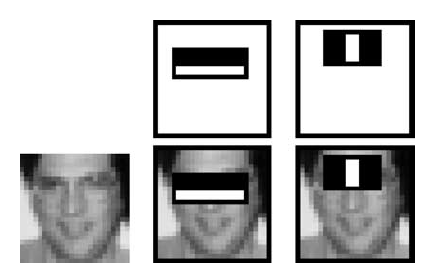
\includegraphics[width=4in]{ViolaJonesFace} 
\caption{Image from Viola and Jones well known paper, Robust Real-Time Face Detection\cite{viola2004robust}}
\end{figure}

	For our purposes, Viola and Jones' specific facial recognition, by design, only works with images of faces. Naturally, though, one would imagine that a similar process to this facial recognition could be used in attempting to recognize other objects in images, like clothing. In theory, we should be able to find prominent features that belong to any given type of clothing item, and use this feature to consistently classify the image.
		
	 As stated above, in images, we count on an item to have one or more identifying features, like a human face. One of the ways that we can find the parts in an image that are likely to be important, and make them more prominent, is by applying a filter to the image. 

	A common example of a filter is the use of a neighbourhood operator, or local operator on pixels in an image. A neighbourhood operator uses an area of pixels around a specific pixel in an image to compute an output value for that pixel. When applied to all pixels across the image, the operator "filters" the image. A neighbourhood operator takes a weighted sum of all pixels in a neighbourhood. It is also known as a correlation, where h(k, l) are labelled the filter coefficients.\cite{szeliski2010computer} 
	
\begin{equation}
g(i,j) = \sum_{k,l} f(i+k,j+l)h(k,l)
\end{equation}
	
	More relevant for the purposes of this paper is the convolutional operator. Convolution is a variation on correlation(filtering) and is both commutative and associative. It is a reversal of the sign of the offsets of the correlation function  g = f * h where h is now an impulse response function.\cite{szeliski2010computer}. To explain this not just in formulas, but with respect to pixels in images, a convolution on a single pixel is done by taking a weighted sum of the pixels in the neighbourhood of this pixel. The weights, and size of the neighbourhood depend on the convolution kernel\cite{RiverTrail}. 
\begin{equation}
g(i,j) = \sum_{k,l} f(k, l)h(i + k, j + l)
\end{equation}
%That's a convolutional operator
	A convolution kernel can be any size, but is usually quite small. Since we only want to use pixels within a certain neighbourhood around a pixel, this makes sense. A convolution kernel too small will not consider any pixels around it, and too large will end up loosing the importance of the pixel itself. A common convolutional operator is the sobel operator, whose 2 convolution kernels are shown in figure 5. This filter is used for edge detection and is very helpful in finding shapes, objects, and defining features in images. Two 3x3 convolution kernels are used to perform this edge detection\cite{Sobel}. On their own, G$_{x}$highlights vertical lines in an image and G$_{y}$ highlights horizontal lines in an image.
\begin{figure}
\centering
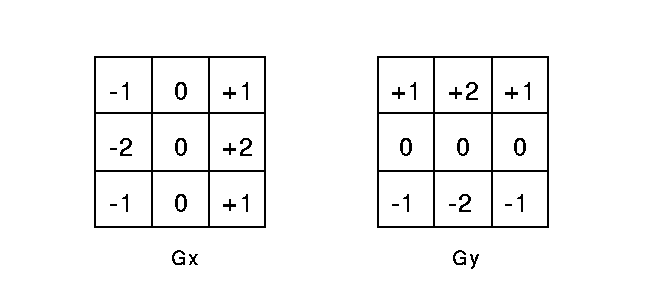
\includegraphics[width=4in]{sobel_operator} 
\caption{Sobel Operator: Convolution Kernels G$_{x}$ and G$_{y}$ $\cite{Sobel}$}
\end{figure}	
	 To apply one convolution kernel across an image, for instance G$_{x}$, we need to inversely apply the weights in the kernel around the neighbourhood of a given pixel (a convolution) and take the sum of these values. In the case of Sobel's G$_{x}$ kernel, the pixel in question will be at (2, 2) or in the middle of the kernel. This weighted sum then becomes the value for that pixel. This is done across all pixels in an image\cite{RiverTrail}. 
	 An example of this can be seen in figure 6. The image on the top shows a high level view of a convolution being applied, and underneath shows a convolution kernel being applied to a set of pixels in the neighbourhood of a number 2 (in the middle of the 3x3 section of pixels).	 
	 
	 What is important to note is that this operation cannot be done on the pixels around the edges or corners of an image, because their neighbourhood is limited. To deal with this problem, often zero padding is added, which adds a border of pixels all with the value 0 around the image. In this way, the original edge pixels in an image can then be part of the convolution. \cite{R. Fisher, S. Perkins, A. Walker and E. Wolfart.} Another approach is to avoid applying the convolution kernel to the outer pixels, and in this case these pixels will essentially be thrown away after the convolution. This should only be done if one is assuming that the pixels around the edge of the image are unimportant, which is often the case.
	 
\begin{figure}
\centering
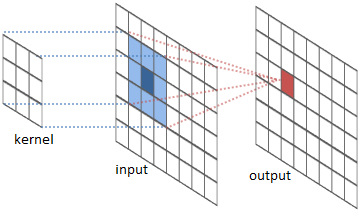
\includegraphics{RiverTrain-ImageConvDiagram} 
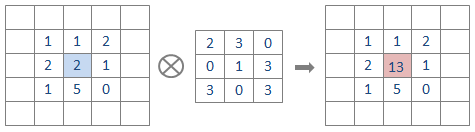
\includegraphics{convolution4}
\caption{A Convolution kernel being applied to an image $\cite{RiverTrail}$}
\end{figure}	 
	 
	 After applying a convolution operator, correlation operator, or any type of filter to an image, we are left with a feature map. A feature map is essentially a filtered image. Since each filter highlights a certain feature, or set of features in the image, a feature map can provide us with a lot of information about what is in an image, and what is important in an image\cite{aurelienMachineLearning}. Having multiple feature maps, which can show us if images have a number of different features, these can then be used to help us learn things about an image.
	
	As outlined above, filters can alter an image in dramatic ways. They can be used for edge detection, to blur photos, to adjust colour, or to sharpen images.\cite{szeliski2010computer}. Filters can play a crucial part in detecting any object in an image, as a feature map helps a computer to recognize certain features in an image. Even so, to manually find which features are important and which filters or convolution kernels work for each object is not always a feasible task. Filters are helpful in discovering features in an image and making them more prominent, but when dealing with 1000 or more images, how do we know which filters to use and what features are important? 
\chapter{Machine Learning}
	Machine Learning can help us "learn" things about these images, namely which filters or convolution kernels work best, without having to manually go through and picking filters for each clothing type. 
	
	Simply put, Machine learning is programming a computer to learn something based on the data itself. People use machine learning to analyze and monitor data much more efficiently than executing it manually. It recognizes patterns, and can be used to learn what people are buying, which emails in your inbox are spam, and in this case, if a pair of jeans is in an image, and indeed which pair of jeans it is. \cite{aurelienMachineLearning}. 

\section{Training Sets and Classifiers}
	Using machine learning algorithms, we can program a computer to learn about almost anything as long as we provide it with enough data, and the right data. For instance, if we want a computer to use machine learning to "learn" if a pair of shoes are present in an image, we have to make sure that we provide it with many images of many different kinds and brands of shoes, in different positions and orientations. These images are called our training set.\cite{aurelienMachineLearning}. The images in the training set are input into a machine learning algorithm called a "classifier"\cite{KubatMachineLearn}. The algorithm then goes through the entire set of images and looks for similar features among all or most of the images. 
	
	Choosing a training set can be difficult, to properly train a machine learning classifier we need (as stated earlier) a lot of the right data. That might be impossible for a small boutique 
with only 100 items in total. Because most people do not have a database with thousands of photos, there must be some resource providing photos to take advantage. And there is. 
	Imagenet \cite(Imagenet) is a website that gives access to millions of pre-classified images, 14,197,122 at this moment, to be exact. An entire database of images of a specific classification can be downloaded, or all images can be accessed by urls. Something like this will be useful for the clothing designer in question. Instead of having to personally take thousands of photographs to have a decent sized training set for the clothing items that this designer has, Imagenet can be used to easily get whatever images are needed, whenever they are needed. Figure 7 shows a screen shot of imagenet in which 1227 images are available and were classified as "Dinner dress, dinner gown, formal, evening gown". If this clothing designer specializes in something like fancy dresses, they can take these images as part of their training set that represents fancy dresses, or any of the labels previously mentioned.
\begin{figure}
\centering
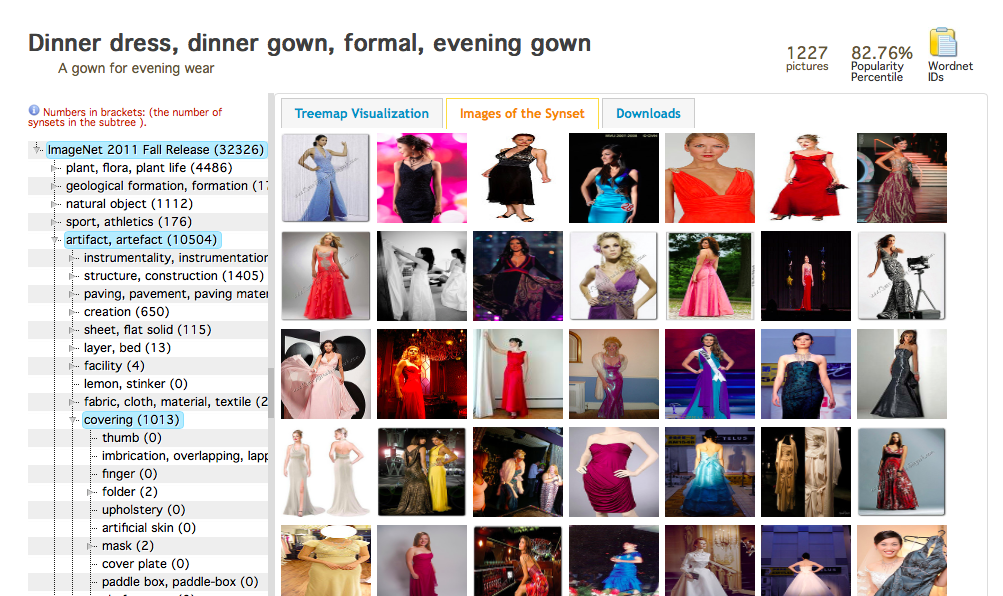
\includegraphics[width=7in]{Imagenet_dress}
\caption{What is returned from Imagenet after searching for dress: http://image-net.org/synset?wnid=n03201638}
\end{figure}	
	Even with the tremendous help of Imagenet\cite(Imagenet) providing a good training set, we need a classifier to recognize (or correctly classify) a clothing item in an image. Once a classifier is trained, it gives us a probability that the image belongs to each of the classes it has been trained on. Whichever probability is the highest, is the predicted class of an item\cite{KubatMachineLearn}. If the designer with a boutique has photos of their clothing ready on hand, the theoretical app and classifier should be able to take images of all of the designer's clothes, and give each image a label, or class. 
	
	Before being able to do this though, the classifier needs to learn the way in which it will get the best results with the data (in this case, images) available. This data is how a machine learning algorithm will be trained, hence the name "training set". After being trained, an algorithm should be able to predict the class of an object in an image, but only for objects that it has already been trained on. In other words, as long as the classifier was trained on dresses, the predicted class, or label of a photo of a dress, should be one that refers to a dress. 
	
	In this case, supervised learning will be used. With supervised learning, the algorithm already knows the class, or label, that each specific data element in the training set belongs to, and makes use of this for training purposes. If a classifier predicts that a data element belongs to the wrong class during the training phase, supervised learning lets the algorithm run again with the same data to attempt to correct its' previous mistakes\cite{aurelienMachineLearning}. Thus, a classifier learns by making predictions on the same training set continuously until it can accurately predict the classes of all or most data elements in the training set. 
	
	How can supervised learning help in predicting which clothing item is in an image? Since we do not have to get everything right the first time with supervised learning, we can use a method that makes mistakes each time (or each epoch) that it iterates through our dataset. When a classifier is in its' training phase, an epoch refers to one iteration through the training data. Depending on the way in which it is trained and with which and how much data, a classifier may need many many training epochs to be properly trained. The number of training epochs needed will depend on the  type of classifier (neural network, nearest neighbour, SVM, etc), the number of possible classes, and the data. So how can we tell when a classifier is properly trained? 
	
	To measure how well a classifier has been trained we use a testing set of data (again, which in this case will be images) in which all elements are different from those in the training set, the classifier will iterate through the testing set. It will keep track of the actual prediction it makes for the element, and the correct prediction. Calculating the error of the previous epoch, and going back to fix the mistakes previously made by the classifier. There must be a type of classifier that make use of this idea.
\chapter{Neural Networks}
	
	Artificial Neural networks are an effective classifier for any data set that needs to be learned, but that will need several (or many) training epochs. The type of neural networks that we're interested in use deep learning which is a subfield of machine learning and Artifical Intelligence. Deep learning uses big data sets and deep neural networks with many hidden layers and neurons\cite{deepMachineMastry}. Like most machine learning algorithms (classifiers)  neural networks take one data element as input (one image in this case), and outputs a probability that this element belongs to each class in a list of classes. What is unique about neural networks is that they are inspired by the human brain. 
	
	Neural networks are made up of a series of layers, and each layer is made up of one of one or more neurons, like the neurons in a human brain. Every neural network has an input layer made up of input neurons, an output layer made up of output neurons, and 1 or more hidden layers composed of hidden neurons.

\begin{figure}
\centering
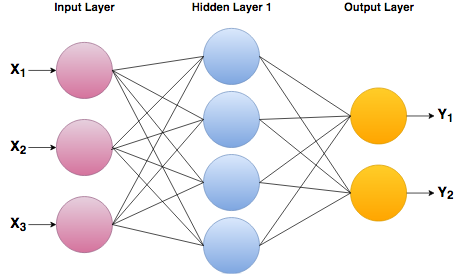
\includegraphics[width=5in]{NeuralNetwork}
\caption{A simple neural network with 3 input neurons, 1 hidden layer with 4 neurons, and 2 output neurons}
\end{figure}
	For the purpose of explanation, an example will be given as shown in figure 8, with only one hidden layer. There are three input neurons, or signals: x$_{1}$, x$_{2}$, and x$_{3}$. Each neuron in the input layer is connected to every neuron in first hidden layer. As can be seen in figure 8, every neuron in one layer is connected to every neuron in the next layer. Each one of these connections has its' own unique weight (weights are important) and a neuron in the first hidden layer takes a weighted sum of all input neurons. This weighted sum is then given to an activation function in each hidden layer. The output of this activation function is the output value of this hidden neuron. This is done for each neuron in the first hidden layer. If there are more hidden layers, the output of the previous hidden layer's neurons are fed into the neurons in these layers as input. This continues until the output layer is reached, where each output neuron represents a specific class and calculates the probability that the input belongs to this class.\cite{KubatMachineLearn}
	
\section{Activation Functions}	
	First of all, every neuron in a neural network except for the input neurons, put their weighted sum of the previous layer into an activation function. An activation function takes this weighted sum mentioned earlier, and adds a bias. Equation 3.1 shows this as the output of any neuron Y. The result of this function determines whether it should activate, or "fire" that neuron. The way in which a neuron uses the result of this function to decide whether it should activate is by declaring a threshold. If Y is over (greater than) this threshold then the neuron fires, if not, the neuron does not fire. This means that if a particular neuron does not fire, it does not contribute to the final output of the network (the classification)\cite{activationMedium}. 
\begin{equation}
Y = \sum  (weight * input) + bias
\end{equation}	
	For a long time, people who worked with neural networks assumed the optimal solution would be one that closely mimics the neurons in a human brain. The activation function used by neurons in the brain is a sigmoid function(Equation 3.2)\cite{KubatMachineLearn}. For many years this was the most commonly used activation function in artificial neural networks. In recent deep learning developments though, it has been discovered that there are several other functions that perform a lot better than the sigmoid function, depending on the type of deep neural network being used. This will be covered in another section.
\begin{equation}
f(\sum) = \frac{1}{1+e^{-\sum}}
\end{equation}		 

\section{Training and Back-propagation}	

 	A Neural network has input neurons and output neurons, hidden layers and activation functions, but how does it learn, and how is it supervised? Back-propagation takes the same input through a network to correct any mistakes made in previous predictions (probabilities of classification). This is where the training set comes in. 
	
	During each Epoch of a training session, each element in the training set is forward-propagated through the neural network. Since we know the correct classification of all elements in our training set, after each epoch we can compute the error in the classification. This can be done using the weights. Since all neurons contribute independently to the classification of the input, each input or hidden neuron in a particular layer has a different weight to carry it to each neuron in the next layer. All weights should be updated by adjusting for the error in the previous epoch. A neural network should improve at predicting the actual class of its input after every training epoch. 
	
	The error of an entire training set's classification can be calculated using accuracy, precision, and recall, but is most commonly calculated using accuracy.  For binary classification (true or false classification) these calculations are done by using the number of true positives, false positives, true negatives and and false negatives. For non-binary classifications (deep neural networks) it is done a little differently. For neural networks, the error is most commonly calculated with MSE, or Mean Squared Error as shown in equation 3.3, where i is the ideal output (or class) for a training element, and a is the actual class, or what the neural network predicted for this element during this training epoch\cite{errorHeaton}.
\begin{equation}
MSE = \frac{\sum\limits_{i=1}^n (i_{n} - a_{n})^2}{n}
\end{equation}		
	Each one of these calculations can tell us how close the network was to making a correct prediction. All of the weights present in a network are adjusted after each epoch based on how much it contributes to the correct classification (its' error). Weights are usually initialized randomly, or randomly within a certain set of values, and then get udated accordingly during training\cite{errorHeaton}. Once a neural network is properly trained, the same weights can be used over and over to make predictions. This process of using error to update weights and train a network is called back-propogation and can help a deep neural network learn almost anything.\cite{KubatMachineLearn} 
	
\chapter{Convolutional Neural Networks}
\section{What are convolutional Neural Networks?}
	Since neural networks can learn almost anything, one would expect that they could learn which objects are in an image, or if an image contains a particular clothing item. Getting back to the theoretical fashion designer, it would be great if there was a type of neural network that could be used to classify images all of their clothing items. This can be done with deep neural networks, but with a bit of an adjustment. A specific type of deep neural network is used for image classification called a convolutional neural network. 

	Convolutional neural networks have a similar flow to other neural networks. The input for this type of network is all pixel values in an image and the output is again the probability that the input belongs to a certain class (for instance, the class "dress"). In this case the output will be the probability that the input image contains a certain object. The hidden layers are where CNNs get more complicated. There are a few possible types of hidden layers. The first and probably most important to the network is a convolutional layer. A convolutional layer applies a number of convolutions to an image each return a feature map\cite{aurelienMachineLearning}. 

\section{Convolutional Layers \& ReLU}
	
	Convolutional layers try to mimic the way that our eyes perceive what is around us. When we look at something, the neurons in our visual cortex are only really focused on a small area of the visual field called the local receptive field. Each neuron has a different local receptive field, although they may overlap. These local receptive fields of specific neurons, which are how our eyes process what they percieve, can be similar to filters in many ways. Some neurons have larger local receptive fields than others, whereas some can focus on and react to lines or other shapes. This is exactly what a convolutional layer attemps to do.\cite{aurelienMachineLearning} 
	
	The first convolutional layer will not have every input neuron connected to every other neuron in the layer like we see in the hidden layers of some other neural networks. Each neuron in the first convolutional layer is connected to a certain number of neurons in the input image which are referred to as the neuron's local receptive field. The weights applied here are similar to a small image in equal size to the local receptive field of a neuron. This small image of weights that are applied to an image is a convolution kernel. A convolution happens here when this kernel is applied to all neurons in the local receptive field of the current neuron. This process is essentially a convolution when applied throughout an entire image. This process of convolution on local receptive fields from a previous layer, helps the network focus on low level features in the beginning stages of forward propogation through the network, and higher level features near the end of the network.\cite{aurelienMachineLearning} 
	
	When all of these convolutions are applied in a convolutional layer, we are left with feature maps (or filtered images) of the previous layer. Because these layers return a number of feature maps, the network learns which features are best at predicting the class of a particular image using back-propogation. A feature which helps in predicting the class will be more heavily weighted in the network. whereas a feature which does not contribute to a prediction will be minimally weighted.
	
	Since neural networks apply an activation function after all data has entered a neuron, we would expect CNNs to do the same. There are several different activation functions that a CNN can use on the image data of a layer, but the most common one is the ReLU function. As mentioned in a previous section, in biological neurons, the sigmoid function gives the best learning results, but with deep neural networks, there are other activation functions that give better results and speed up the training time.\cite{krizhevsky2012imagenet} 
	
	For CNNs and some other deep neural networks, The ReLU (Rectified Linear Unit) function is preferred over other functions like sigmoid, because it does not saturate for positive values (sigmoid does) and gives 0 when any input is negative. Since the output of some neurons will undoubtably be 0 after computing ReLU, we can assume that many neurons will end up dropping out, or having no effect on the classification. This is okay for our purposes, but there are some good variations on ReLU that make sure neurons do not get killed or left out during the rest of the training process. \cite{aurelienMachineLearning} 
 \begin{equation}	
 (x) = max(0, x)%RELU function
 \end{equation}
 
	One variation on ReLU activation is LeakyReLU. It uses a hyperparameter (or tuneable parameter) \( \alpha \) to determine the "leakage" of the function. In this case, the neuron may become temporarily inactive, but may eventually contribute to the network again, which is an improvement over ReLU. Another variation on ReLU is PReLU (Parametric Leaky ReLU) which takes the hyperparameter in LeakyReLU and makes it a parameter learned with backpropogation during the network's training. These variations perform well when the training set is large, but may overfit on smaller datasets. Since the dataset being considered for this project is quite small, ReLU will be fine for our training purposes. The activation function is important to note here because each convolutional layer in a CNN is usually followed by a layer in which the activation function (ReLU) is applied to all neurons in the previous layer.\cite{aurelienMachineLearning} 
 \begin{equation}
LeakyReLU_\alpha(z) = max(\alpha z, z)
  \end{equation} 
  
 \section{Max Pooling Layer}

	The next hidden layer commonly used in convolutional neural networks, and other deep neural networks is a pooling layer. A pooling layer is used to summarize a large amount. In the case of images, this means reducing the size of the image, while still keeping certain parts or features of the image.\cite{aurelienMachineLearning}. What these features are will determine what type of pooling layer is used. In most CNNs, max pooling layers are used to keep the most prominent features in an image, which is usually desirable when attempting to recognize objects. 
\begin{figure}
\centering
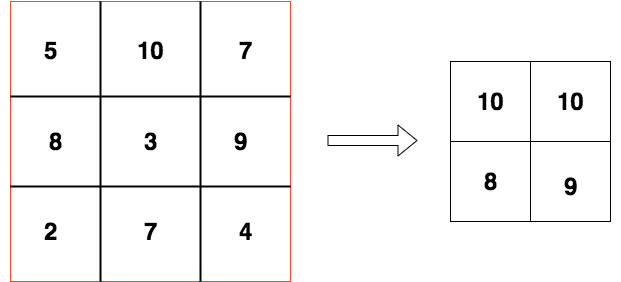
\includegraphics[width=7in]{max_pooling}
\caption{max pooling applied to a 3x3 section of pixels using a 2x2 kernel for pooling}
\end{figure}		
	Max pooling layers summarize the image data by taking the largest pixel value in a group of pixels and using this to represent the group (shown in figure 4.1) . Doing this across an entire image gives a smaller image with less noise. Max pooling layers are usually in between or after convolutional layers (after ReLU has been computed for the convolutional layer). Throughout the network the classification of an image becomes more clear, so it makes sense that after each convolution, we pool the feature maps for the most prominent pixels, which gets us closer and closer to finding the most important and defining features in an image. 

 \section{Fully Connected Layers and Architectures}
	
	The last pooling layer is usually followed by two or more fully connected layers which again will use ReLU as an activation function. Fully connected layers are actually quite simple and are often placed at the end of the network. They work like the layers in a generic neural network as explained earlier in the paper. Each neuron in a previous layer is connected to every neuron in the fully connected layer, hence the name "fully connected"\cite{LeonardoFully}. These layers help with training by giving the data from the last pooling layer a chance to propagate through a few more hidden layers before outputting a prediction. 
	
	Finally, as we already know, the output layer in a convolutonal neural network is similar to the output layer in most neural networks. Depending on the number of classes, the network returns a probability that the image belongs to each class, and the highest probability is the predicted class. 
	
	A typical Convolutional neural network has an input layer, a few convolutional layers (each followed by a pooling layer) followed by two or three connected layers. Even though there is a general flow and consensus on which layers go where, the number of layers is dependent on the task itself and is usually discovered by trying different CNN (Convolutonal Neural Network) architectures.
	
	There are a few famous CNN architectures. These include LeNet-5, AlexNet, GoogLeNet, and ResNet. All of these architectures and their layers are outlined in the O'Rielly Book: Machine Learning with Scikit-Learn and TensorFlow.\cite{aurelienMachineLearning}. As an example, the AlexNet architecture, which won the 2012 ImageNet ILSVRC challenge and had the least amount of error by nine percent, was developed in 2012. A simple table outlining its' architecture can be seen in figure 5.2
\begin{figure}
\centering
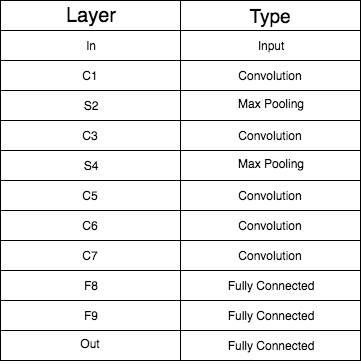
\includegraphics[width=3in]{alex_net_arch}
\caption{Simple view of AlexNet architecture inspired by Table 13.2 on page 367$\cite{aurelienMachineLearning}$}
\end{figure}		

\chapter{TensorFlow}
	We can in fact build something to recognize images of clothing and classify images that a fashion designer takes of their clothing. Convolutional neural networks and the right training and testing set a computer or an app on a phone can be trained to recognize images in photos. This is theoretically sound but how can it be implemented? Implementing a simple neural network that works as a binary classifier is a lot of work even for an experienced programmer. Someone looking to create an app that matches clothing in images may not have the time or experience to create a convolutional neural network from scratch. 
\section{What is TensorFlow?}
	TensorFlow is a library that allows for building deep neural networks (including CNNs) in Python (which is now also available in C++, Java, and Go). More formally, as defined in the TensorFlow documentation,  "TensorFlow is an open source software library for numerical computation using data flow graphs. Nodes in the graph represent mathematical operations, while the graph edges represent the multidimensional data arrays (tensors) communicated between them. The flexible architecture allows you to deploy computation to one or more CPUs or GPUs in a desktop, server, or mobile device with a single API."\cite{tensorFlow}
	
	TensorFlow was originally developed with the intention of being used to build and work with Deep Neural Networks, but can now be used for other types of computation as well. With TensorFlow, defining layers, weights, and training a network is quite straightforward. The TensorFlow API provides methods for all of these things which take parameters specific to the graph or neural network being built. The documentation also provides tutorials on how to use TensorFlow. There are tutorials on building convolutional neural networks which can help tremendously with learning how they are actually implemented. A portion of this tutorial is shown in figure 6.1. It can also be seen that when using TensorFlow, "tensors" are created.\cite{tensorFlow}
\begin{figure}
\centering
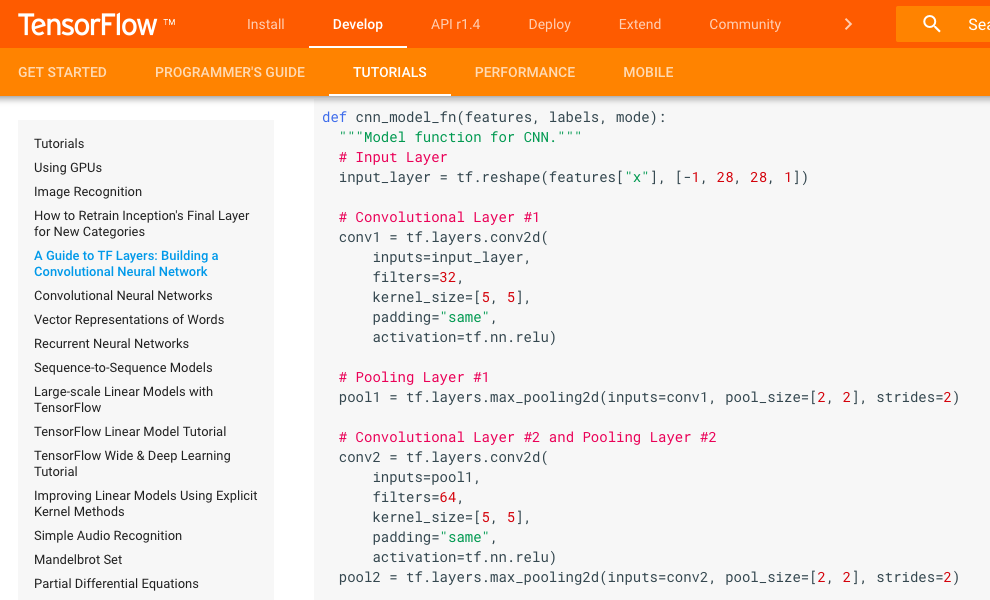
\includegraphics[width=5in]{tensorflow_cnn}
\caption{A portion of code from a  CNN tutorial using TensorFlow$\cite{tensorFlow}$}
\end{figure}	
\section{What is a Tensor}
	Along with the previous definition taken from the TensorFlow documentation on the home page of TensorFlow's website, it is also defined as: "A framework to define and run computations involving tensors."\cite{tensorFlow}. Tensors generalize matrices and vectors, possible in higher dimensions. The are implemented as n-dimensional arrays. When using TensorFlow to write a program, a tensor is the object that is used by the rest of the program throughout the duration of the program, and is defined as a tf.Tensor. Usually, when a tensor is instantiated, it is only partially defined, as it may or not yet contain the data that the program will be working with. A tensor can be easily defined with its' two properties, a data type and a shape\cite{tensorFlow}.
	
	The data type will be consistent throughout every element of the array. The shape is the number of dimensions of the tensor, and the size of each of these dimensions. Each dimension contains an array of the given by the shape. There are several types of tensors, some of the most commonly used are Variable, . Tensors also have a rank which is determined by their shape. To see the value of a tensor we can use the .eval() function. As explained in the documentation, the rank of a tensor refers to an entity in math as shown in Figure 6.2. This table makes tensors a lot easier to visualize and understand\cite{tensorFlow}.
\begin{figure}
\centering
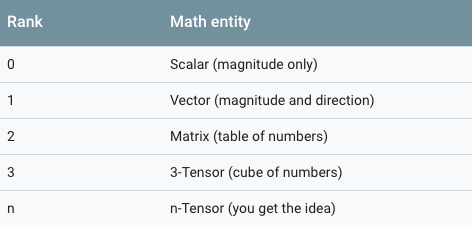
\includegraphics[width=4in]{tf_rank}
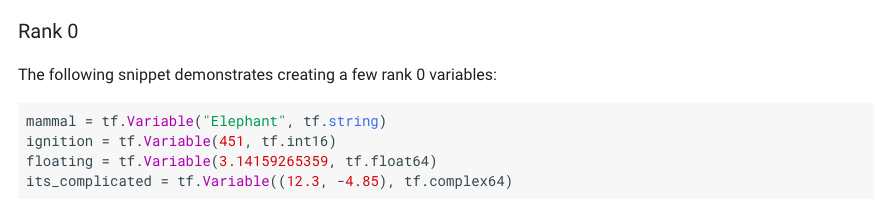
\includegraphics[width=7in]{rank0}
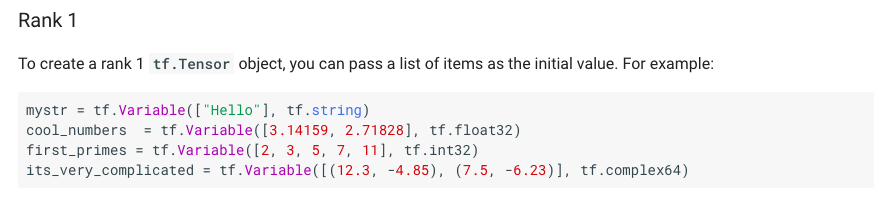
\includegraphics[width=7in]{rank2}
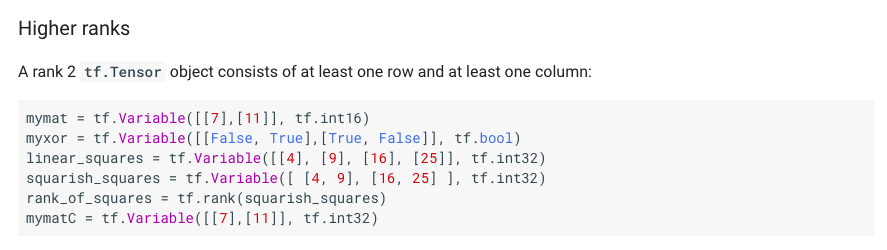
\includegraphics[width=7in]{rank1}
\caption{Tensor ranks and the mathematical entities they represent followed by examples of tensors of different ranks.$\cite{tensorFlow}$}
\end{figure}	
\section{Using TensorFlow to Build a CNN}
	TensorFlow can be used to build a convolutional neural network with any amount or sequence of layers. A set of images of any size can be used as long as the shape of the tensors are defined properly. After installing and importing TensorFlow, starting with the training phase, some tensors need to be defined to hold the data being worked within the network. For example, for a training set of 200 images, if all images in the training set are known to be 100x100 pixels and all images are RGB, we can define a tensor holding the input to a CNN as a tensor of type tf.float32. This means the pixel data of each image will be represented as a 3D array where each pixel is an element of a 2-D array and is represented a three element array with the RGB values. The definition of this tensor is shown in the following four lines of Python code.
\begin{verbatim}
batch_size = 200
img_height = 100
img_width = 100
num_channels = 3
input = tf.placeholder(tf.float32, shape=[batch_size, img_width, img_height, num_channels])
\end{verbatim}

	A tensor must also be defined during the training phase containing the true class of each element in the training set, these true classes will be used to calculate the error of a training epoch, by seeing how many elements in the training set were given the correct prediction by the classifier (the CNN).
\begin{verbatim}
labels = tf.placeholder(tf.int32, shape=(batch_size))
\end{verbatim}
	
	After having defined placeholders for the input and its' classes, the network itself can be built. As mentioned in Chapter 5, a convolutional neural network has an input layer, convolutional layers, max pooling layers, and fully connected layers (one of which is the output layer). This may seem like a lot of work to write all of the code for these layers, and it can be to put it all together, but TensorFlow makes defining the layers easy. Luckily, the TensorFlow API defines layers of all of these types that can be used when building a convolutional neural network. For example, we can define the layers of a simple CNN (where the input layer is an element in the training set) with the following lines of code, assuming all variables being used as parameters for layers have been previously defined. We can also assume here that all initial weights for trainings have been defined and generated.
	
\begin{verbatim}
#first convolutional layer
layer_conv_1 = tf.nn.conv2d(input=input, filter=weights_kernel, strides=[1, 1, 1, 1], padding='SAME')

#apply relu activation function to first convolutional layer
layer_ReLU_1 =  tf.nn.relu(layer_conv_1)

#pool the output of layer_ReLU_1
layer_max_pool_1 = tf.nn.max_pool(value=layer_ReLU_1, ksize=[1, 2, 2, 1], strides=[1, 2, 2, 1], padding='SAME')

#second convolutional layer
layer_conv_2 = tf.nn.conv2d(input=layer_max_pool_1, filter=weights_kernel, strides=[1, 1, 1, 1], padding='SAME')

#apply relu activation function to second convolutional layer
layer_ReLU_2 = tf.nn.relu(layer_conv_2)

#pool the output of layer_ReLU_2
layer_max_pool_2 = tf.nn.max_pool(value=layer_ReLU_2, ksize=[1, 2, 2, 1], strides=[1, 2, 2, 1], padding='SAME')

#first fully connected layer which takes layer_max_pool_2 as input and flattens the previous layer
layer_fully_connected_1 = tf.contrib.layers.flatten(layer_max_pool_2)
layer_fully_connected_1 = tf.layers.dense(layer_fully_connected_1, size)
layer_fully_connected_1 = tf.layers.dropout(layer_fully_connected_1, rate=dropout, training=is_training)

#second fully connected layer
layer_fully_connected_2 = tf.layers.dense(layer_fully_connected_1, size)
layer_fully_connected_2 = tf.layers.dropout(layer_fully_connected_2, rate=dropout, training=is_training)

#third fully connected layer which is the output layer
layer_fully_connected_out = tf.layers.dense(layer_fully_connected_2, num_classes)
\end{verbatim}

	Now that these layers are defined, the input can be given to the CNN and the network can be trained. The TensorFlow documentation also contains tips and tutorials on training neural networks\cite{tensorFlow}. After the network is trained, we can use these layers and the weights which were determined during training as a classifier, to make predictions about images.
	
\chapter{Unanswered Questions}
	It has been shown that using TensorFlow, a convolutional neural network can be implemented by making full use of their high level API. This could be used in an app to classify images of clothing, as mentioned before, and this app could be used by a fashion designer. This fashion designer wants to be able to use this app give all of their images a classification, and use this label to match it to another image. This image which is input into the app (or the CNN) will be provided by a customer. Even with a straightforward way to build a convolutional neural network, and a theoretical app using the network as a classifier, there are still a few unanswered questions.
	
\section{Using a Pretrained CNN}
	The first question is: how can this neural network be trained, if the boutique that wants to use it only has a few hundred photos? This question has already been answered in part, but now that the way in which a classifier can be built and trained has been discussed, this question can be answered in more detail. 
	
	Since ImageNet can be used as a resource for a training set of images, and convolutional neural networks can be build without too much trouble, there have been many people who have taken the initiative to train networks on ImageNet's vast selection of images. But what does this mean for a brand new network that has not been trained yet? As mentioned before, the process of training a neural network is to come up with the proper set of weights that when applied within the network, create an accurate classifier. Many of these people who have trained CNNs on ImageNet have provided their set of weights for anyone to use. This is so helpful for anyone who does not need a classification specific to their needs, and who wants to use a CNN to simplify what is in an image. 
	
	This means that an app with these capabilities can simply take a photo of a sneaker, for instance, as input, and give it a label telling the user that is a sneaker. This is useful, but does not match an image to another image like the designer of a boutique may want. An image needs to be matched with another image in this case so that a user can find an item that looks like something they saw in a store or on the street, and if a small boutique has a similar item, the user will be told where they can get this item. The problem here though, is that CNNs (and neural networks in general) do not match images, they classify them. 

\section{Possibilities for More Convolutional Neural Networks}
	There are several possibilities when it comes to image matching, but this paper will look at implementing one of these possibilities. In terms of progress made with the theoretical fashion designer and app, we can now give a photo of a clothing item a label tells us what this item is. This label and the opportunity to use weights provided by a network trained on ImageNet should not go to waste.
	
	As mentioned in the introduction to this paper, a boutique wanting to use something like this may only have 100 items, and only 4 types of items: dresses, shirts, shoes, and jeans. This leaves only 25 items of each type. 
	
	The first step to image matching might be to narrow down the options. If an image is labeled as a dress, there are 25 possible matches for this dress. It also must be considered that if this boutique expands that there may be 50 dresses, or maybe even 100.  Because the options for potential matches needs to be narrowed down, four convolutional neural networks can be created. One trained on images of dresses, one trained on images of shirts, one trained on images of shoes, and one trained on images of jeans.
	
	This idea of having four separate networks may seem like a lot of work. As discussed though, only one network is needed. This one network must be trained on the four data sets with different images, and the weights from each of the four training sessions can then be used as a classifier. To get closer to the goal of image matching, each of these types of items must be broken down into several categories so that only a few images containing very similar items remain. 
	
	To use an example, there are many types of dresses, but this boutique only carries long evening gowns, summer beach dresses, short party dresses, and puffy ball gowns. In this case, the neural network specific to dresses will be trained to classify an image that has already been labeled a dress as either an evening gown, summer beach dress, short party dress, or puffy ball gown. Since the boutique currently only has 25 dresses in total, separating the dresses based on these four types, and using this specifically trained network to classify an image, there can now only be a few possible matches to deal with for the an input image. 
\section{Possibilities for a Training Set}
	
	An important question here, is how do we train these CNNs with more specific classifications to be able to perform this task with only a few images of each of these more focused types? Setting the problem of size of training set aside for the moment, and assuming a couple of hundred photos taken from image net will suffice for training purposes, how do we choose the images on which these four networks will be trained?
	
	Since the number of images is limited here, and the type of item so specific, it would make sense to train a network in a way in which it does not waste time trying to locate where the object is in an image with a busy background. A solution to this problem may be to make sure all backgrounds of the images of an entire training set are identical. But this may seem counter productive. In chapter one it was mentioned that if images of a specific class have a white background, this white background will be learned as a feature of the item itself.
	
	Why might a white background actually work in this case? If every single image in a training set has a white background, theoretically a convolutional neural network cannot in any way use the background to learn about a specific item. In this case, features of the item itself must be used to differentiate between the types of items because the background is consistent in all images.
\begin{figure}
\centering
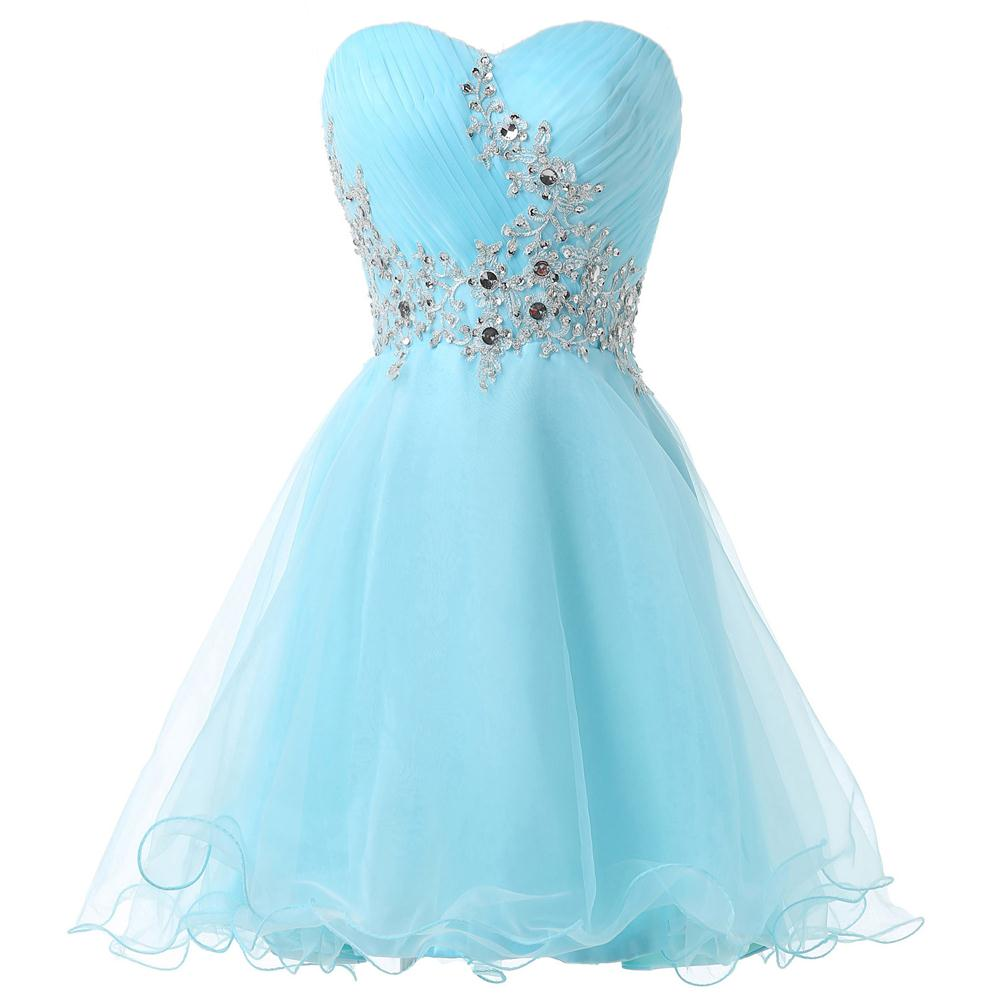
\includegraphics[width=3in]{short_party_dress}
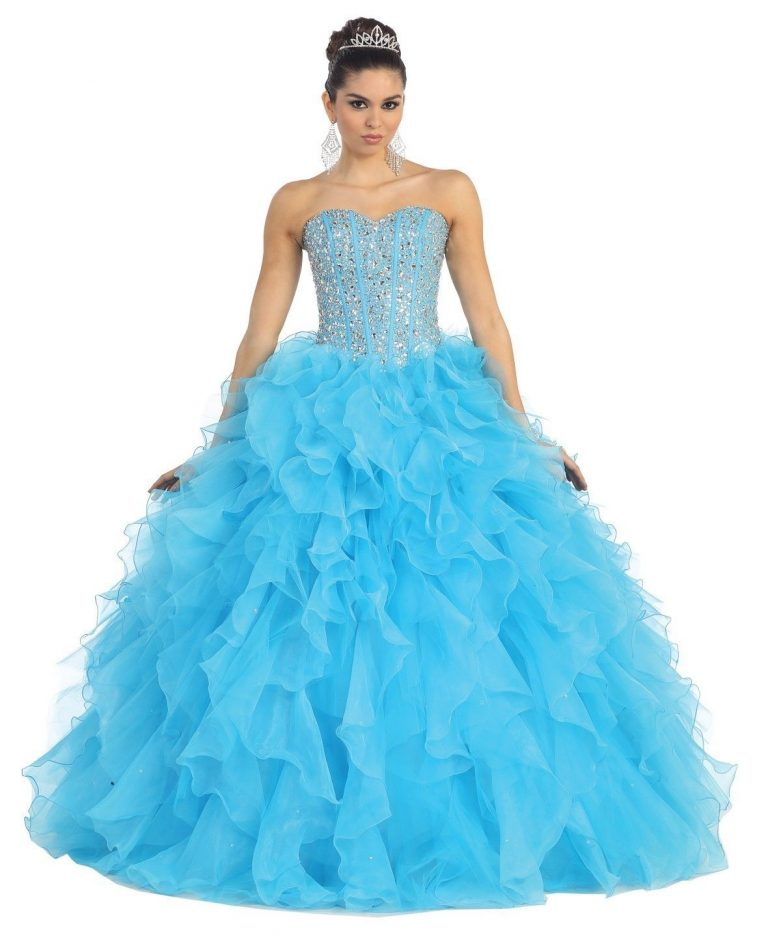
\includegraphics[width=3in]{ball_gown}
\caption{An image of a short party dress and a puffy ball gown both with white backgrounds. Left Image: $\cite{partyDressImage}$. Right Image:  $\cite{ballGownImage}$.}
\end{figure}		
	This may or may not work for images with different backgrounds, which are most images. A solution to this problem would be to only allow images with white backgrounds (which is very limiting) or to write a program which finds the object in an image and creates a white background around the image. Even in the possible creation of a white background for every input image, the object must be very prominent in the image.  If this does work though, it is an option as a way to narrow down the possible matches of an image without having a large training set.
	
\section{Possibilities for Image Matching}
	After Narrowing possible matches for a customer's input image to only a few, the closest match still needs to be found. There are several different ways this could be done, and different ways could be used depending on the specifics of the type of item. For instance, we know that SIFT\cite{lowe1999object} can recognize rigid objects, so it could be the way in which shoes are matched. 
	
	Since dresses are usually deformable objects, a method that may work for dresses is the nearest neighbour algorithm. The name of this machine learning algorithm actually tells us a lot about it. The simple idea here is to find the k (where k is an integer) closest elements to one element, x,  in a data set. The most prominent class among these k closest elements will become the class of x. In Theory, the part of the algorithm which determines the "nearest" elements to x, should be able to determine the image that most closely matches an input image that has been labeled by the more focused and specific CNN, and only has a few possible matches.\cite{nearestNeighbour}
%I actually found a couple of papers on this topic but they couldn't be accessed for free.	

\chapter{Experiments and Conclusion}
[This section will be filled in in the coming weeks as I finish up attempting the implementation of methods mentioned in Chapter 7]
		
\bibliographystyle{plainyr}
\bibliography{References}
\end{document}

